\chapter{String Theory and M-Theory}

This chapter follows Leonard Susskind's third lecture in the supplementary string theory sequence. He does not begin with the string spectrum itself. Instead he stages two preliminaries that will be needed almost immediately: first a very fast harmonic-oscillator review, meant mainly to fix notation for string modes, and then a review of the special spin content of massless particles. We follow that order closely. Where the blackboard layout matters, we keep it visible; where the blackboard is cropped or heuristic, we stabilize the mathematics from the transcript. In that spirit these notes explicitly preserve the lecture of Leonard Susskind and the supporting curation work of LazyingArt LLC and Video2Book.

\section{Rapid Harmonic-Oscillator Review for String Modes}

Susskind begins by reminding us that each normal mode of an open string behaves like a harmonic oscillator. The only slightly odd feature is the normalization inherited from the string calculation: a factor of \(4\) sits in the denominator, and he insists that we keep it exactly as it appears rather than tidying it away. The mode number \(n\) is the same \(n\) that appears in the cosine mode \(\cos n\sigma\); it labels how many half-waves fit along the interval \(0\leq \sigma \leq \pi\).

\begin{figure}[t]
\centering

\includegraphics[width=0.62\textwidth]{lecture_03_figure_02.png}
\caption{Harmonic oscillator energy and Lagrangian.}
\end{figure}

The blackboard frame makes the pedagogical point very clearly: the energy and the Lagrangian are built from the same quadratic pieces, with only the sign of the potential term changed. The right-hand labels are cropped in the frame, but the transcript fixes them unambiguously:
\begin{align}
E_n &= \frac{\dot X_n^{\,2}}{4}+\frac{n^2X_n^{\,2}}{4}, \\
L_n &= \frac{\dot X_n^{\,2}}{4}-\frac{n^2X_n^{\,2}}{4}.
\end{align}
From the Lagrangian one recovers the equation of motion of an oscillator of frequency \(n\). That is the whole point of the review: every string mode is an oscillator, and its frequency is precisely its mode number.

Once we decide to quantize, the first step is to pass from the Lagrangian to the Hamiltonian. At the blackboard Susskind suppresses the subscript \(n\) for a moment and writes the single-oscillator coordinate simply as \(x\). The conjugate momentum is
\begin{equation}
p=\frac{\partial L}{\partial \dot x}=\frac{\dot x}{2},
\end{equation}
so that \(\dot x=2p\). Substituting back into the energy gives the Hamiltonian
\begin{equation}
H=p^2+\frac{n^2x^2}{4}.
\end{equation}
Nothing deep has happened yet. We have only rewritten the same oscillator in the language appropriate for quantum mechanics.

\section{Hamiltonian, Ladder Operators, and the Return to the String}

Now comes the familiar oscillator trick. The Hamiltonian is a sum of squares,
\begin{equation}
H=p^2+\left(\frac{nx}{2}\right)^2,
\end{equation}
and Susskind uses the standard heuristic factorization
\begin{equation}
H \sim \left(\frac{nx}{2}+ip\right)\left(\frac{nx}{2}-ip\right).
\end{equation}
This is not meant as a polished statement about operator ordering. It is the blackboard-level guide to the right linear combinations of \(x\) and \(p\).

The normalization is fixed by the commutator. With \(\hbar=1\),
\begin{equation}
[x,p]=i.
\end{equation}
Therefore
\begin{align}
\left[\frac{nx}{2}+ip,\frac{nx}{2}-ip\right]
&=
-\frac{ni}{2}[x,p]+\frac{ni}{2}[p,x] \\
&=
-\frac{ni}{2}(i)+\frac{ni}{2}(-i) \\
&= \frac{n}{2}+\frac{n}{2}=n.
\end{align}
The would-be ladder operators therefore have commutator \(n\), not \(1\). The remedy is immediate: divide by \(\sqrt n\). That gives
\begin{align}
a^- &= \frac{1}{\sqrt n}\left(\frac{nx}{2}+ip\right)
= \frac{\sqrt n\,x}{2}+\frac{i}{\sqrt n}p, \\
a^+ &= \frac{1}{\sqrt n}\left(\frac{nx}{2}-ip\right)
= \frac{\sqrt n\,x}{2}-\frac{i}{\sqrt n}p,
\end{align}
with
\begin{equation}
[a^-,a^+]=1.
\end{equation}
Susskind is careful about the interpretation: the sign in the formula does not by itself tell us which operator raises the energy and which lowers it. The commutator does. The convention above is chosen so that \(a^+\) raises the energy and \(a^-\) lowers it.

In three space dimensions, if the string is moving with large momentum along the \(z\)-axis, the independent oscillations are transverse. There are therefore two copies of the oscillator, one in the \(x\)-direction and one in the \(y\)-direction. We introduce a second pair of operators,
\begin{align}
b^- &= \frac{\sqrt n\,y}{2}+\frac{i}{\sqrt n}p_y, \\
b^+ &= \frac{\sqrt n\,y}{2}-\frac{i}{\sqrt n}p_y,
\end{align}
and similarly
\begin{equation}
[b^-,b^+]=1.
\end{equation}

\begin{figure}[t]
\centering

\includegraphics[width=0.62\textwidth]{lecture_03_figure_03.png}
\caption{Commutators for the \(a\)- and \(b\)-oscillator modes.}
\end{figure}

The frame is especially useful here because it preserves the board hierarchy: first the commutators, then the operator definitions beneath them. In cleaned form the basic block is
\begin{equation}
[a^-,a^+]=1,\qquad [b^-,b^+]=1,\qquad [x,p]=i.
\end{equation}

From the definitions of \(a_n^\pm\) we can solve back for the coordinates. Adding the two equations eliminates the momentum and gives
\begin{equation}
a_n^++a_n^-=\sqrt n\,x_n,
\end{equation}
so
\begin{equation}
x_n=\frac{a_n^++a_n^-}{\sqrt n},\qquad
y_n=\frac{b_n^++b_n^-}{\sqrt n}.
\end{equation}
This step matters. It brings us back from abstract oscillator algebra to the string itself.

The open string is parameterized by \(\sigma\in[0,\pi]\). Its transverse coordinates are expanded in cosine modes,
\begin{align}
x(\sigma,\tau) &= \sum_n x_n(\tau)\cos n\sigma, \\
y(\sigma,\tau) &= \sum_n y_n(\tau)\cos n\sigma.
\end{align}
The cosine basis is appropriate because the endpoint condition is
\begin{equation}
\partial_\sigma x\big|_{\sigma=0,\pi}=0,\qquad
\partial_\sigma y\big|_{\sigma=0,\pi}=0,
\end{equation}
so the slopes vanish at the ends. Substituting the oscillator coordinates gives
\begin{align}
x(\sigma,\tau) &= \sum_n \frac{a_n^++a_n^-}{\sqrt n}\cos n\sigma, \\
y(\sigma,\tau) &= \sum_n \frac{b_n^++b_n^-}{\sqrt n}\cos n\sigma.
\end{align}
This is the point of the whole exercise: once the string coordinates are written in terms of creation and annihilation operators, the quantum mechanics becomes transparent. We can see immediately what a given operator does to the energy of a state.

\begin{figure}[t]
\centering
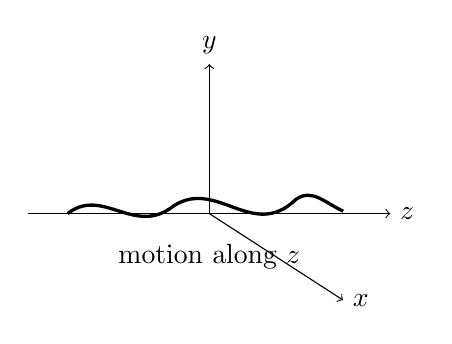
\begin{tikzpicture}[scale=1.0]
\draw[->] (-2.3,0)--(2.3,0) node[right] {$z$};
\draw[->] (0,0)--(0,1.9) node[above] {$y$};
\draw[->] (0,0)--(1.7,-1.1) node[right] {$x$};
\draw[very thick] (-1.8,0) .. controls (-1.35,0.35) and (-0.95,-0.30) .. (-0.45,0.10)
                  .. controls (0.10,0.45) and (0.55,-0.35) .. (1.10,0.18)
                  .. controls (1.30,0.32) and (1.45,0.15) .. (1.70,0.03);
\draw (0,-0.55) node {motion along \(z\)};
\end{tikzpicture}
\caption{The string is taken to move with large momentum along the \(z\)-axis. The independent oscillations are transverse, in the \(x\)- and \(y\)-directions.}
\end{figure}

\subsection{Question \& Answer}

\paragraph{Question.} Do the coefficients \(x_n\) depend on \(\sigma\)?

\paragraph{Answer.} No. All of the \(\sigma\)-dependence sits in the trigonometric factors \(\cos n\sigma\). The coefficients \(x_n\) and \(y_n\) are Fourier coefficients, and in the present discussion they depend on the time variable \(\tau\). That is why the dots in the oscillator formulas are really \(\tau\)-derivatives: the modes vibrate in time, while the cosine functions encode the shape along the string.

\section{Massive Versus Massless Spin}

The second preliminary concerns spin. For a massive particle of spin \(J\), the familiar counting is
\begin{equation}
N_{\mathrm{massive}}(J)=2J+1.
\end{equation}
Thus a massive spin-\(1\) particle has three states, a massive spin-\(2\) particle has five states, and so on. But Susskind wants us to notice immediately that massless particles do not follow this pattern. In the massless case,
\begin{equation}
N_{\mathrm{massless}}(0)=1,\qquad N_{\mathrm{massless}}(s>0)=2.
\end{equation}
For spin \(1\), instead of three states \((+1,0,-1)\), only two remain. For spin \(2\), instead of five states, again only two remain.

The clean way to understand this is to compare a massive particle with a massless one moving along, say, the \(z\)-axis. Reflection symmetry already tells us that if maximal positive helicity exists, maximal negative helicity must exist as well. The real question is whether states in between are compulsory.

For a massive particle they are compulsory. One may move to the particle's rest frame. Once the particle is at rest, one can rotate the spin direction and then boost back to a moving frame. That procedure produces states whose spin is no longer purely parallel or antiparallel to the direction of motion. In particular, a spin-\(1\) particle must then carry the three states \(+1\), \(0\), and \(-1\).

For a massless particle this route is blocked. There is no rest frame. One can never bring a massless particle to rest, rotate it there, and then boost it back. The obstruction is precisely what allows the intermediate helicity states to disappear. The only states that must remain are the states of maximal and minimal helicity.

\subsection{Question \& Answer}

\paragraph{Question.} Why do massless particles have only two polarization states?

\paragraph{Answer.} Because the argument that generates the intermediate states requires a rest frame. A massive particle can be brought to rest, rotated, and then boosted back, so the full \(2J+1\) multiplet must be present. A massless particle cannot be brought to rest. The rotate-then-boost construction never gets started, and it is therefore consistent for the particle to carry only the two extreme helicity states.

\section{Photon Polarization as the Model Case}

The familiar example is the photon. The polarization of a photon is always transverse to the direction of motion. If the photon travels along the \(z\)-axis, then its polarization lies in the \(xy\)-plane. One may choose a linear basis, which we denote by \(|x\rangle\) and \(|y\rangle\), or a circular basis,
\begin{equation}
|R\rangle = |x\rangle + i|y\rangle,\qquad
|L\rangle = |x\rangle - i|y\rangle.
\end{equation}
These are lecture-level basis states; we do not normalize them here because normalization is not the point. The point is the transformation law. The circular combinations are helicity eigenstates. They are the two physical states of the photon.

The linear states are also perfectly good states, but they are not eigenstates of angular momentum along the direction of motion. For example, \(|x\rangle+|y\rangle\) is simply a linearly polarized state rotated by \(45^\circ\) in the transverse plane. The complex unit \(i\) is what turns a linear polarization basis into the circular basis.

\begin{figure}[t]
\centering
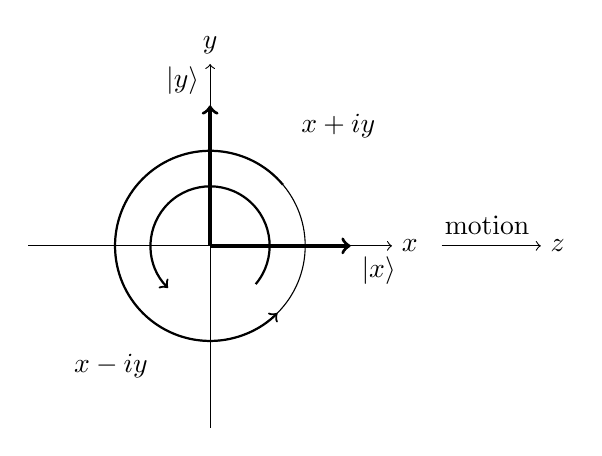
\begin{tikzpicture}[scale=1.05]
\draw[->] (-2.2,0)--(2.2,0) node[right] {$x$};
\draw[->] (0,-2.2)--(0,2.2) node[above] {$y$};
\draw[very thick,->] (0,0)--(1.7,0) node[below right] {$|x\rangle$};
\draw[very thick,->] (0,0)--(0,1.7) node[above left] {$|y\rangle$};
\draw (0,0) circle (1.15);
\draw[thick,->] (40:1.15) arc (40:315:1.15);
\draw[thick,->] (-40:0.72) arc (-40:225:0.72);
\draw (1.55,1.45) node {$x+iy$};
\draw (-1.20,-1.45) node {$x-iy$};
\draw[->] (2.8,0)--(4.0,0) node[right] {$z$};
\draw (3.35,0.25) node {motion};
\end{tikzpicture}
\caption{Linear and circular polarization in the plane transverse to the motion.}
\end{figure}

The same logic already hints at the graviton. A massless spin-\(2\) particle again has only two states, not five. It is useful, though only as an analogy, to think of the two graviton helicities as built from two photons of like helicity. That is a mnemonic for the helicity structure, not an ontological claim that a graviton is literally made of two photons.

\subsection{Question \& Answer}

\paragraph{Question.} Does linear polarization mean zero angular momentum?

\paragraph{Answer.} Not as an eigenvalue statement. A linearly polarized photon is a quantum superposition of the two helicity states. Its average angular momentum along the direction of motion may vanish, but an actual measurement yields one helicity or the other. There is no third photon state with zero helicity along the axis.

\section{The First Excited Open-String States and the Photon-Like Interpretation}

Now Susskind turns to the actual target of the lecture: the low-lying spectrum of the open string. The preliminary work is complete. We know how to build the oscillator states, and we know what it means for a relativistic particle to have only two transverse polarizations.

Let \(|0\rangle\) denote the unexcited string state. This is not empty space. It is a single string whose oscillators are all as quiet as quantum mechanics permits:
\begin{equation}
a_n^-|0\rangle = 0,\qquad b_n^-|0\rangle = 0
\end{equation}
for every mode \(n\). Susskind does not immediately assign it a definite mass. He leaves its mass-squared flexible and writes
\begin{equation}
m^2(|0\rangle)=m_0^2.
\end{equation}
The important point is that oscillator energy, in this light-cone-like bookkeeping, contributes to mass-squared rather than directly to mass.

What is the cheapest excitation? Since the \(n\)th oscillator adds \(n\) units, the least expensive step is to excite the \(n=1\) mode. There are two such states,
\begin{equation}
a_1^+|0\rangle,\qquad b_1^+|0\rangle,
\end{equation}
and they have the same mass-squared,
\begin{equation}
m^2 = m_0^2+1.
\end{equation}
Any linear combination has the same value of \(m^2\). In particular, the circular combinations
\begin{equation}
\left(a_1^+ \pm i\,b_1^+\right)|0\rangle
\end{equation}
have the same transformation properties as the two helicity states of a massless spin-\(1\) particle.

This is the decisive step. The operators \(a_1^+\) and \(b_1^+\) came from the transverse coordinates \(x\) and \(y\), so they transform as the components of a transverse vector. There are only two such states. There is no third polarization state. By the entire preceding discussion, that is impossible for a massive spin-\(1\) particle and perfectly natural for a massless one. Therefore the first excited open-string state must be massless. The condition is
\begin{equation}
m_0^2+1=0.
\end{equation}

This is already enough to identify the state as photon-like, or more generally gauge-boson-like. It would be premature to call it \emph{the} photon, because string theory generically contains many photon-like states and their detailed interpretation is model-dependent. But it is certainly a massless spin-\(1\) object with exactly two transverse polarizations.

Historically this was once viewed as an annoyance rather than a triumph, because the earliest versions of string theory were being used as models of hadrons, and one does not want a massless meson. But within the logic of the present lecture it is a triumph first, and then, almost immediately, a disaster.

\section{The Tachyonic Ground-State Disaster}

The disaster is sharp. If the first excited state is massless, then the ground state must satisfy
\begin{equation}
m_0^2=-1
\end{equation}
in the lecture's units. The open string has produced exactly the right photon-like excitation, but only by forcing the state beneath it to have negative mass-squared. That is the point at which Susskind says, only half jokingly, that we ought to throw the theory away.

\subsection{Question \& Answer}

\paragraph{Question.} Does negative mass-squared mean faster-than-light propagation?

\paragraph{Answer.} Not in the sense that matters physically. The old terminology ``tachyon'' came from the naive reading of a relativistic dispersion relation, but the modern lesson is different. Negative mass-squared signals that we have expanded the theory around an unstable configuration. The real problem is instability of the vacuum, not a practical way of sending signals faster than light.

To see why the older language arose, recall first the group-velocity rule
\begin{equation}
v_g=\frac{dE}{dp}.
\end{equation}
For a nonrelativistic particle,
\begin{equation}
E(p)=\frac{p^2}{2m},
\qquad
\frac{dE}{dp}=\frac{p}{m},
\end{equation}
which is just the ordinary velocity. For a relativistic particle, with \(c=1\),
\begin{equation}
E=\sqrt{p^2+m^2},
\qquad
\frac{dE}{dp}=\frac{p}{\sqrt{p^2+m^2}}.
\end{equation}
This is manifestly less than \(1\) when \(m^2>0\). If one naively replaces \(m^2\) by a negative quantity, the denominator can become smaller than \(p\), and that is what tempted people to interpret the state as superluminal.

But Susskind insists that this is not the right interpretation. The right interpretation comes from the wave equation and the effective potential. In the stable case,
\begin{equation}
\omega^2 = k^2 + m^2,
\end{equation}
and the corresponding quadratic piece of the field energy is
\begin{equation}
\mathcal{E}_\phi
=
\frac12\left[(\partial_t\phi)^2+(\partial_x\phi)^2+m^2\phi^2\right].
\end{equation}
The last term is the crucial one. If \(m^2>0\), then displacing \(\phi\) costs potential energy and the field oscillates back, just as an ordinary harmonic oscillator does. If instead \(m^2<0\), the quadratic potential near \(\phi=0\) is inverted:
\begin{equation}
V(\phi)\propto -|m|^2\phi^2.
\end{equation}
Then \(\phi=0\) is not a stable minimum at all. It is the top of a hill.

\begin{figure}[t]
\centering
\begin{tikzpicture}[scale=0.95]
\begin{scope}[xshift=-3.6cm]
\draw[->] (-2,0)--(2,0) node[right] {$\phi$};
\draw[->] (0,-0.2)--(0,2.2) node[above] {$V$};
\draw[domain=-1.7:1.7,smooth,variable=\x,thick] plot ({\x},{0.42*\x*\x});
\draw (0,-0.55) node {stable};
\end{scope}
\begin{scope}[xshift=3.6cm]
\draw[->] (-2,0)--(2,0) node[right] {$\phi$};
\draw[->] (0,-2.2)--(0,0.5) node[above] {$V$};
\draw[domain=-1.7:1.7,smooth,variable=\x,thick] plot ({\x},{-0.42*\x*\x});
\draw (0,-2.65) node {tachyonic};
\end{scope}
\end{tikzpicture}
\caption{Positive mass-squared gives an ordinary quadratic potential; negative mass-squared turns the quadratic term upside down and makes \(\phi=0\) unstable.}
\end{figure}

That is why the pendulum and domino analogies matter. A perfectly balanced pencil can sit forever if it is exactly balanced, but the slightest push sends it away. Likewise for a chain of coupled inverted pendulums: the instability propagates outward with an advancing front, but the front does not outrun the wave speed of the system. One gets an instability, not a causal violation.

So the open bosonic string has taught us two things at once. First, it has produced a massless photon-like excitation that looks exactly right. Second, it has done so in a theory whose ground state is unstable. The latter problem is what later leads us toward superstring theory.

\section{Rotating Strings, Joining and Splitting, Closed Strings, and Gravity}

Having reached the photon-like open-string state, Susskind changes direction. To get to the graviton one must discuss something new: closed strings. Before that, however, he pauses to remind us that a free string can carry more than the simplest vibrational excitations. It can also rotate. As in ordinary mechanics, a string rotating about its center of mass carries angular momentum, and in the quantum theory each additional unit of angular momentum costs additional energy. This fits smoothly with the oscillator picture: the spectrum contains higher and higher excitations carrying more and more spin.

The new ingredient is interaction. For open strings the basic process is simple and qualitative. If two endpoints come to the same point in space, there is an amplitude for them to join and form a single open string. By reversibility, the opposite process must also exist: a single open string may break and form two endpoints. The small parameter that controls these processes is the string coupling constant. Susskind emphasizes that, at this level, it is the same basic coupling for all string states; the differences in observed interaction probabilities arise because different strings spend different amounts of time in contact.

\begin{figure}[t]
\centering
\begin{tikzpicture}[scale=0.95]
\begin{scope}[xshift=-5.5cm,yshift=2.1cm]
\draw (-1.4,0.3)--(-0.3,0.3);
\draw (-1.4,-0.3)--(-0.3,-0.3);
\draw[->] (0,0)--(0.8,0);
\draw (1.0,0)--(2.1,0);
\draw (0.35,-0.85) node {\small open + open \(\to\) open};
\end{scope}

\begin{scope}[xshift=1.5cm,yshift=2.1cm]
\draw (-2.1,0)--(-1.0,0);
\draw[->] (-0.8,0)--(0,0);
\draw (0.2,0.3)--(1.3,0.3);
\draw (0.2,-0.3)--(1.3,-0.3);
\draw (0.35,-0.85) node {\small open \(\to\) open + open};
\end{scope}

\begin{scope}[xshift=-5.5cm,yshift=-1.1cm]
\draw (-1.3,0)--(0.0,0);
\draw[->] (0.2,0)--(1.0,0);
\draw (1.7,0) circle (0.55);
\draw (0.35,-1.0) node {\small open bites its tail};
\end{scope}

\begin{scope}[xshift=1.5cm,yshift=-1.1cm]
\draw (-2.0,0.4) circle (0.35);
\draw (-2.0,-0.4) circle (0.35);
\draw[->] (-1.2,0)--(-0.3,0);
\draw (0.5,0) circle (0.55);
\draw (0.25,-1.0) node {\small closed + closed \(\to\) closed};
\end{scope}

\begin{scope}[xshift=-2.0cm,yshift=-4.0cm]
\draw (-2.4,0) circle (0.35);
\draw (-0.8,0)--(0.7,0);
\draw[->] (1.0,0)--(1.8,0);
\draw (2.0,0)--(3.8,0);
\draw (0.75,-0.95) node {\small closed + open \(\to\) open};
\end{scope}
\end{tikzpicture}
\caption{Qualitative interaction rules used in the lecture: joining, splitting, self-closing, pure closed-string interaction, and absorption of a closed string by an open string.}
\end{figure}

Now comes the decisive topological observation. An open string can encounter its own tail. If the joining interaction is allowed at all, then nothing prevents the string from joining to itself and forming a closed loop. Therefore an interacting theory of open strings inevitably contains closed strings. There is no escape from this.

The converse statement is different. A theory that begins with closed strings need not contain open strings. Closed strings have their own interaction channel: two closed strings may meet, exchange partners, and continue as closed strings without ever producing open endpoints. Thus one may have a pure closed-string theory, but not a pure interacting open-string theory.

This is already enough to show why gravity is unavoidable. The first low-lying excitation of the open string was photon-like. By the same sort of argument, the first interesting low-lying excitation of the closed string turns out to be graviton-like. Once closed strings are inevitable, gravity is inevitable. There is more: a closed string can be absorbed by an open string, leaving an open string behind. In the graviton interpretation that process is the absorption of a graviton by a non-graviton. Likewise a closed string can interact with another closed string. In this simple-minded but powerful sense, everything can absorb a graviton, and that is why everything gravitates.

\subsection{Question \& Answer}

\paragraph{Question.} Why must interacting open-string theories contain closed strings, while pure closed-string theories need not contain open strings?

\paragraph{Answer.} Because the open-string joining rule applies whenever endpoints meet, including the case in which a single open string meets its own endpoint configuration and closes on itself. The very interaction that lets open strings talk to each other therefore generates closed strings automatically. Closed strings, however, possess a direct closed-string interaction channel, so they can interact among themselves without ever producing open endpoints. Hence closed-only theories are possible, but open-only interacting theories are not.

\section{Summary}

The lecture was built as a staged argument. First, each string mode was reset to a harmonic oscillator with the lecture's peculiar but important normalization. Then the oscillator algebra was turned back into the string coordinates themselves. Next came the crucial representation-theoretic fact: a massless particle with spin \(s>0\) has only two helicity states. Once these two preliminaries are in hand, the first excited open-string states can only be interpreted as a massless, photon-like transverse vector. That success forces the ground state to have negative mass-squared, so the open bosonic string carries a tachyon and therefore an unstable vacuum. Finally, the move from free open strings to interacting strings makes closed strings unavoidable, and once closed strings are unavoidable, gravity is unavoidable as well. The unresolved issue of units, which Susskind repeatedly postpones, remains postponed here as well; it belongs to the next stage of the story.